
\begin{figure}
\centering
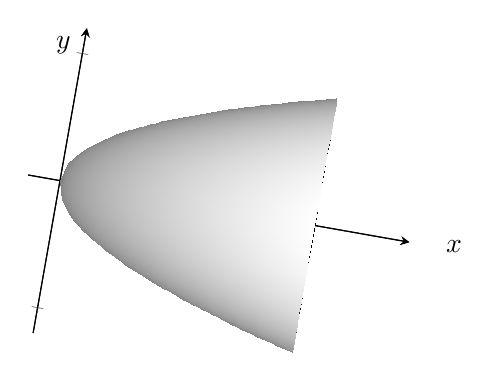
\begin{tikzpicture}
\begin{axis}[axis equal image, axis lines=middle,enlargelimits=true,
    clip=false,
    colormap/blackwhite,
%shader=flat,
shader=interp,
view={10}{90},
    %y dir=reverse,
    %axis on top, 
axis z line=none,
xlabel={$x$},ylabel={$y$},xmax=5,xlabel style={at={(current axis.right of origin)},anchor=west}
    ]
    % sym. Torus:
            \addplot3[domain=0:4,y domain=0:360, samples=50,
            surf,z buffer=sort
            ]
            ({x} ,
            {sqrt(x)*sin(y)},
            {sqrt(x)*cos(y)});
\end{axis}
\end{tikzpicture} 
%

\end{figure}


